\documentclass[conference]{IEEEtran}
\usepackage{algorithm}
\usepackage{algpseudocode}
\usepackage{listings}
\usepackage{xcolor}
\usepackage{amsmath}
\usepackage{graphicx}
\usepackage{float}
\usepackage{booktabs}
\usepackage{url}
\usepackage{circuitikz} % This also loads tikz
\usepackage{array}

\lstset{
  basicstyle=\ttfamily\small,
  keywordstyle=\color{blue}\bfseries,
  commentstyle=\color{green!40!black},
  stringstyle=\color{red},
  numbers=none,                     % no numbers
  numberstyle=\scriptsize\ttfamily, % more readable numbers
  numbersep=8pt,                    % add spacing from code
  xleftmargin=1.5em,                % indent code so numbers don’t overlap
  frame=single,
  breaklines=true,
  breakatwhitespace=true,
  tabsize=2,
  showstringspaces=false,
  captionpos=b,
  keepspaces=true                   % preserve spacing properly
}

\title{Implementation of Cross-Platform Data Transmission Systems: A Comparative Study of Wired Serial and Bluetooth Low Energy (BLE) Bridging using nRF5340}

\author{
\IEEEauthorblockN{Bhargav K, Harsha B J}
\IEEEauthorblockA{
Department of Electrical Engineering\\
IIT Hyderabad\\
Email: ee25btech11013@iith.ac.in, ee25btech11026@iith.ac.in}
}

\begin{document}

\maketitle
\begin{abstract}
This paper presents the design and implementation of a cross-platform bidirectional data transfer system, enabling seamless telemetry and file exchange between a Linux host and an Android mobile environment. The study contrasts a baseline wired serial connection against a wireless embedded bridge utilizing the Nordic Semiconductor nRF5340 SoC.

In the wireless implementation, the nRF5340 functions as a protocol converter, bridging USB-CDC (ACM) serial data to Bluetooth Low Energy (BLE) packets via the Nordic UART Service (NUS). To mitigate data corruption caused by control character interpretation in the UART stack, a Base64 encoding scheme was integrated, successfully enabling the transmission of binary assets (images, PDFs) with 100\% data integrity.
\end{abstract}

\section{Hardware Requirements}
\begin{itemize}
    \item \textbf{Development Board:} Nordic Semiconductor nRF5340 DK.
    \item \textbf{Smartphone:} Android device with Termux and Serial Bluetooth Terminal App.
    \item \textbf{PC:} Linux machine (Ubuntu).
    \item \textbf{Cable:} Micro USB cable(data transfer and power).
\end{itemize}

\section{System Model and Hardware Architecture}

To facilitate cross-platform communication, the system architecture acts as a bridge between standard wired protocols and wireless Bluetooth Low Energy (BLE). 

\subsection{System Model}
The system model comprises three primary nodes: the Linux Host PC, the nRF5340 Development Kit (acting as the bridge), and the Android Client Device. Data originates from the Linux terminal, passes through a virtual COM port via USB-CDC, is processed by the nRF5340's application core, and is finally transmitted wirelessly using the Nordic UART Service (NUS) over BLE to the smartphone (and vice versa).

\begin{figure}[htbp]
\centering
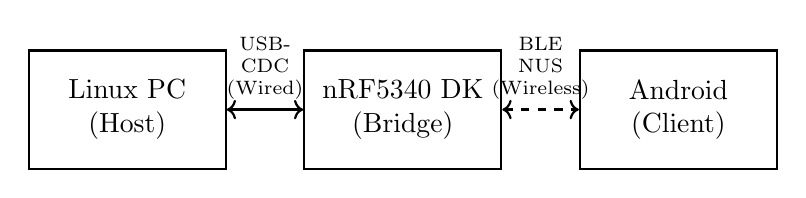
\begin{tikzpicture}[node distance=2cm, auto, thick]
    % Nodes
    \node[draw, rectangle, minimum width=2.5cm, minimum height=1.5cm, align=center] (pc) {Linux PC\\(Host)};
    \node[draw, rectangle, minimum width=2.5cm, minimum height=1.5cm, align=center, right of=pc, node distance=3.5cm] (nrf) {nRF5340 DK\\(Bridge)};
    \node[draw, rectangle, minimum width=2.5cm, minimum height=1.5cm, align=center, right of=nrf, node distance=3.5cm] (phone) {Android\\(Client)};

    % Arrows
    \draw[<->] (pc) -- node[above, align=center, font=\scriptsize] {USB-\\CDC \\ (Wired)} (nrf);
    \draw[<->, dashed] (nrf) -- node[above, align=center, font=\scriptsize] {BLE \\ NUS\\(Wireless)} (phone);
\end{tikzpicture}
\vspace{0.2cm}
\caption{System Model for Cross-Platform Data Transmission.}
\label{fig:system_model}
\end{figure}

\subsection{Hardware Connections}
The physical hardware setup is deliberately minimalist, leveraging the onboard Interface MCU (IMCU) of the nRF5340 DK. The Linux PC is connected directly to the \textbf{IMCU USB} port of the development kit. This single cable serves a dual purpose: it supplies power to the SoC and provides the physical transport layer for the serial UART-to-USB bridge.

\begin{figure}[htbp]
\centering
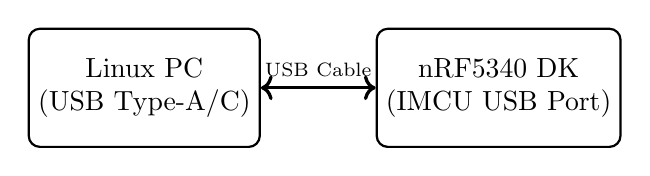
\begin{tikzpicture}[node distance=2.5cm, auto, thick]
    % Nodes
    \node[draw, rectangle, rounded corners, minimum width=2.5cm, minimum height=1.5cm, align=center] (pc) {Linux PC\\(USB Type-A/C)};
    \node[draw, rectangle, rounded corners, minimum width=2.5cm, minimum height=1.5cm, align=center, right of=pc, node distance=4.5cm] (nrf) {nRF5340 DK\\(IMCU USB Port)};

    % Connection
    \draw[<->, line width=1.2pt] (pc) -- node[above, font=\scriptsize] {USB Cable} (nrf);
\end{tikzpicture}
\vspace{0.2cm}
\caption{Hardware Connection Diagram.}
\label{fig:hardware_connections}
\end{figure}

\section{Transferring Binary Files via Base64}
The Nordic UART Service (NUS) is designed for character-based data streams. Attempting to send raw binary files (e.g., \texttt{.jpg}, \texttt{.png}, \texttt{.pdf}) directly will result in data corruption due to control characters and null bytes. To transfer these files, we must encode them into a text-safe format using Base64. \\
\subsection{1. Concept Overview}
The process involves three stages:
\begin{enumerate}
    \item \textbf{Sender (Linux):} Encodes the binary file into a Base64 text string.
    \item \textbf{Transmission:} The text string is sent over the USB-to-Bluetooth bridge.
    \item \textbf{Receiver (Smartphone/PC):} Receives the text string and decodes it back into the original binary format using standard Base64 decoding tools.
\end{enumerate}

\subsection{2. Technical Constraints}
\begin{itemize}
    \item \textbf{Overhead:} Base64 encoding increases the file size by approximately 33\%.
    \item \textbf{Speed:} Bluetooth Low Energy (BLE) has a limited bandwidth. The observed speed is around 4.5 kB/second. Transferring large files (e.g., $>$ 1MB) may take several minutes.
    \item \textbf{Buffer:} Ensure the receiving device does not sleep during transfer, as BLE connections may drop if the radio is idle for too long.
\end{itemize}

\section{Nordic Provided Examples for UART Text Transfer}

Nordic Semiconductor provides an official sample application for Bluetooth-based 
serial communication as part of the nRF Connect SDK. The \texttt{peripheral\_uart} 
sample, located at:

\begin{center}
\texttt{nrf/samples/bluetooth/peripheral\_uart}
\end{center}

\noindent demonstrates the use of the \textbf{Nordic UART Service (NUS)}, a 
custom BLE GATT service that emulates a serial port over Bluetooth Low Energy. 
This sample is designed specifically for text-based data streaming and serves 
as the official reference implementation for UART-to-BLE bridging on Nordic 
hardware.

\subsection{What the Official Sample Provides}
The stock \texttt{peripheral\_uart} sample includes the following baseline 
capabilities:
\begin{itemize}
    \item Bidirectional text data transfer between a UART interface and a BLE 
    central device.
    \item Asynchronous UART handling via Zephyr's \texttt{uart\_async\_adapter}.
        \item A basic two-LED status system: \textbf{LED1} blinks to indicate the 
    firmware is running, and \textbf{LED2} lights up when a BLE connection is 
    established.
    \item Optional BLE security via passkey confirmation using the onboard buttons.
    \item A generic startup message: \textit{``Starting Nordic UART service sample''} 
    printed over UART on boot.
\end{itemize}

\subsection{Limitations of the Official Sample}
While functional, the official sample lacks the following:
\begin{itemize}
    \item No runtime feedback on how much data has been transferred.
    \item No visual indication that data is actively being received over BLE 
    (LED2 only reflects connection state, not data activity).
    \item The startup banner provides no useful runtime configuration information 
    to the developer.
\end{itemize}

\noindent These limitations motivated the enhancements described in the 
following section.

\section{Modifications and Improvements to the Peripheral UART Sample}

\subsection{Enhancement 1 -- Informative Startup Banner}

The original startup message printed over UART was a generic placeholder string: 
\textit{``Starting Nordic UART service sample''}. This was replaced with a concise 
yet more informative banner that displays the configured buffer size at boot time:

\begin{verbatim}
NUS Bridge Ready [40]
\end{verbatim}

\noindent
This gives immediate confirmation that the firmware is running and displays the 
active buffer configuration, which is useful during testing and debugging without 
exceeding the 40-byte UART transmit buffer limit.

\subsection{Enhancement 2 -- BLE Data Activity Indicator via LED}

A visual data activity indicator was added using \textbf{LED3} (\texttt{DK\_LED3}). 
When the device receives data over the BLE NUS (Nordic UART Service) connection, 
LED3 turns ON when the first BLE NUS packet is received. Each subsequent packet resets the delayed-work timer, keeping LED3 ON continuously. LED3 turns OFF only after the data stream stops and the timer finally expires — giving a real-time "transfer active" indicator.

\noindent
This was implemented using Zephyr's \textbf{delayable work queue} mechanism 
(\texttt{k\_work\_delayable}), which schedules the LED off event without blocking 
the BLE callback thread, making it non-intrusive to data throughput.

\noindent
\textbf{Why this is better than a simple \texttt{k\_sleep()}:} Calling 
\texttt{k\_sleep()} inside a BLE callback can stall the thread and cause missed 
packets. The work queue approach offloads the LED shutdown to a background task, 
keeping the data path completely unaffected.

\section{Industry Applications of Nordic SoCs}
Nordic Semiconductor SoCs are widely adopted in commercial IoT sectors. Notable examples include:
\begin{itemize}
    \item \textbf{Wearables:} The \textit{Ultrahuman Ring Air} and \textit{Dayton Smartwatch} utilize the nRF52 series for biometric tracking (ECG, Sleep Index).
    \item \textbf{Medical Healthcare:} Devices such as \textit{PulseTape} utilize Nordic chips for continuous ECG monitoring, prioritizing low power consumption for extended battery life.
    \item \textbf{Smart Home:} Significantly, the \textit{eCozy 2.0 Smart Thermostat} employs the \textbf{nRF5340}—the exact SoC utilized in this project—to handle complex connectivity protocols like Matter and Bluetooth Mesh.
\end{itemize}

\section{Conclusion}
This project successfully demonstrated the implementation of a robust, bidirectional wireless data transfer system utilizing the Nordic Semiconductor nRF5340 System-on-Chip. By configuring the nRF5340 as a bridge between a USB-CDC (Serial) interface and the Bluetooth Low Energy (BLE) Nordic UART Service (NUS), we established a seamless communication link between a Linux-based PC and an Android mobile environment.

While the UART protocol is inherently text-based, implementing a Base64 encoding strategy enabled the error-free transmission of complex binary files (images, PDFs) over the link. The comparative analysis between direct wired connections and the nRF5340-based solution highlights the flexibility of BLE for embedded applications. While wired connections offer higher raw throughput, the nRF5340 implementation provides a reliable, low-power wireless alternative suitable for IoT remote debugging, field telemetry, and file exchange.

% --- APPENDICES ---
\appendices
\section{Software and Toolchains Installations}

\subsection{1. Update \& Install System Dependencies}
First, update the package manager and install the core dependencies required by the Zephyr build system (CMake, Ninja, Python, etc.).

\begin{lstlisting}[language=bash]
sudo apt update
sudo apt upgrade -y
sudo apt install --no-install-recommends -y \
    git cmake ninja-build gperf \
    ccache dfu-util device-tree-compiler wget \
    python3-dev python3-pip python3-setuptools python3-tk python3-wheel xz-utils file \
    make gcc gcc-multilib g++-multilib libsdl2-dev
\end{lstlisting}

\subsection{2. Set up Python Virtual Environment \& Install West}
Modern Linux distributions enforce PEP 668, which restricts global `pip` installations. The Zephyr build system requires a dedicated Python virtual environment.

\begin{lstlisting}[language=bash]
# Create a virtual environment in the home directory
python3 -m venv ~/zephyr-venv

# Activate the virtual environment
source ~/zephyr-venv/bin/activate

# Install west inside the virtual environment
pip3 install -U west
\end{lstlisting}
\noindent \textbf{Note:} You must run \texttt{source \textasciitilde/zephyr-venv/bin/activate} every time you open a new terminal to build the project.

\subsection{3. Initialize nRF Connect SDK (v3.2.2)}
Create a workspace directory and initialize the specific SDK version used for this project.

\begin{lstlisting}[language=bash]
mkdir ~/ncs
cd ~/ncs

# Initialize the SDK pointing to version v3.2.2
west init -m https://github.com/nrfconnect/sdk-nrf --mr v3.2.2

# Download the code
west update

# Export CMake package for Zephyr
west zephyr-export
\end{lstlisting}

\subsection{4. Install Python Dependencies}
With the virtual environment activated, install the specific Python requirements for the Zephyr kernel, the nRF SDK, and the bootloader.

\begin{lstlisting}[language=bash]
pip3 install -r zephyr/scripts/requirements.txt
pip3 install -r nrf/scripts/requirements.txt
pip3 install -r bootloader/mcuboot/scripts/requirements.txt
\end{lstlisting}

\subsection{5. Install the Zephyr SDK Toolchain}
Download and install the cross-compiler toolchain (Zephyr SDK 0.16.8) required to compile code for the nRF5340 on NCS v3.2.x.

\begin{lstlisting}[language=bash]
# Download the Zephyr SDK Bundle
cd ~
wget https://github.com/zephyrproject-rtos/sdk-ng/
releases/download/v0.16.8/
zephyr-sdk-0.16.8_linux-x86_64.tar.xz

# Extract the archive
tar xvf zephyr-sdk-0.16.8_linux-x86_64.tar.xz

# Run the setup script
cd zephyr-sdk-0.16.8
./setup.sh -c
\end{lstlisting}

\subsection{6. Install nRF Command Line Tools}
Finally, install the J-Link drivers and \texttt{nrfjprog} to enable flashing the board over USB.

\begin{lstlisting}[language=bash]
# Navigate to the download directory
cd ~/Downloads

# Install the .deb package (replace filename with actual version)
sudo dpkg -i nrf-command-line-tools*.deb

# Fix any missing dependencies
sudo apt install -f
\end{lstlisting}

\subsection{Verification}
Verify the installation by checking the versions of the flashing and build tools.

\begin{lstlisting}[language=bash]
nrfjprog --version
west --version
\end{lstlisting}

\section{Project Execution Procedure}

This section details the procedure to compile, flash, and test the \texttt{peripheral\_uart} sample application using the command line interface.

\subsection{1. Workspace Initialization}
Before building, ensure the workspace is correctly set up. If you have not created a specific project folder yet, navigate to:
Target Board: \texttt{nrf5340dk/nrf5340/cpuapp}.
\begin{lstlisting}[language=bash]
cd ~/ncs/v3.2.2
source zephyr/zephyr-env.sh
\end{lstlisting}

\subsection{2. Building the Firmware}
\textbf{Important Note:} Before building, ensure that the default \texttt{main.c} file in the sample directory has been replaced with the custom \texttt{main.c} code provided in the project repository\footnote{\url{https://github.com/gadepall/nordic/blob/98d3648fbc7c7dbd8c8d82ef259fdef46a244059/File_Transfer/codes/main.c}}.

\noindent Target Board: \texttt{nrf5340dk/nrf5340/cpuapp}.
\begin{lstlisting}[language=bash]
west build -b nrf5340dk/nrf5340/cpuapp nrf/samples/bluetooth/peripheral_uart
\end{lstlisting}

\subsection{3. Flashing the Board}
Once the build completes successfully, flash the binary to the nRF5340 development kit.

\begin{enumerate}
    \item Connect the nRF5340 DK to the PC via the \textbf{IMCU USB} port (Interface MCU).
    \item Run the flash command:
\end{enumerate}

\begin{lstlisting}[language=bash]
cd ~/ncs/v3.2.2/nrf/samples/bluetooth/peripheral_uart
west flash
\end{lstlisting}

\noindent If successful, the terminal will display \texttt{Flashing completed}.


\section{File Transfer : Linux Terminal \& Android Serial App}

This section details the procedure to verify bidirectional text transfer using a Linux terminal on the PC side and the \textbf{Serial Bluetooth Terminal} app on an Android device.

\subsection{1. Linux Setup (Receiver/Sender)}
On the Ubuntu machine, we interact with the nRF5340 board through its virtual serial port.

\begin{enumerate}
    \item Connect the nRF5340 DK to the PC via the \textbf{IMCU USB} port.
    \item Open a terminal window and list the USB devices to identify the board (usually \texttt{ttyACM0} or \texttt{ttyACM1}).
\begin{lstlisting}[language=bash]
ls /dev/ttyACM*
\end{lstlisting}
    \item Open the serial connection using \texttt{minicom} with a baud rate of \textbf{115200}.
\begin{lstlisting}[language=bash]
# Replace ttyACM1 with your actual port
sudo minicom -D /dev/ttyACM1 -b 115200
\end{lstlisting}
    \item The terminal screen will clear and wait for input. (Press \textbf{Reset} on the board if you want to see the boot log).
\end{enumerate}

\subsection{2. Android Setup (Serial Bluetooth Terminal)}
We use a dedicated terminal app to act as the Bluetooth Central device.

\begin{enumerate}
    \item \textbf{Install App:} Download and install \textbf{Serial Bluetooth Terminal} (by Kai Morich) from the Google Play Store.
    \item \textbf{Open App:} Launch the application.
    \item \textbf{Scan:}
    \begin{itemize}
        \item Tap the menu (three lines) in the top-left corner.
        \item Select \textbf{Devices}.
        \item Tap the \textbf{Bluetooth LE} tab (important: do not use the Classic Bluetooth tab).
        \item Tap \textbf{Scan} at the top.
    \end{itemize}
    \item \textbf{Connect:} Locate the device named \textbf{Nordic\_UART\_Service} in the list and tap it to connect. The terminal screen should show ``Connected''.
\end{enumerate}

\subsection{3. Verifying File Transfer (Text Streaming)} \label{text}

This section details the procedure to transfer entire text files between the Android device and the Linux machine using the Nordic UART Service.

\subsubsection{Smartphone to Linux (Sending a File)}
To send a text file stored on the phone and save it directly to the Linux host:
\begin{enumerate}
  \item Ensure the devices are connected via the \textbf{Serial Bluetooth Terminal} app.
  \item On the Linux terminal, instruct \texttt{minicom} to capture the incoming serial data to a file by pressing \textbf{Ctrl+A}, followed by \textbf{L}.
 \item When prompted, enter a filename (e.g., \texttt{received\_file.txt}) and press \textbf{Enter}.
 \item On the Android app, tap the \textbf{Menu} icon (three lines) or the \textbf{Upload/Folder} icon.
  \item Select \textbf{Send File}, then browse and select the desired \texttt{.txt} file.
  \item \textbf{Result:} The content of the file will stream into the open \texttt{minicom} session and be written directly to the capture file on the PC.
  \item Once the transfer is complete, safely close and save the file in \texttt{minicom} by pressing \textbf{Ctrl+A}, followed by \textbf{L}, and selecting \textbf{Close}.
\end{enumerate}


\subsubsection{Linux to Smartphone (Sending a File)}
To send a text file from the Linux machine to the phone, we cannot just type in the terminal. We must pipe the file directly to the device port.

\begin{enumerate}
    \item Open a \textbf{new} terminal window (keep the \texttt{minicom} session open in the first window to monitor the connection).
    \item Create a dummy text file to send:
\begin{lstlisting}[language=bash]
echo "This is a test file sent from Linux." > test_file.txt
\end{lstlisting}
    \item Use the \texttt{cat} command to redirect the file into the USB serial port:
\begin{lstlisting}[language=bash]
# Replace ttyACM1 with your actual port
sudo sh -c 'cat test_file.txt > /dev/ttyACM1'
\end{lstlisting}
    \item \textbf{Result:} The content of \texttt{test\_file.txt} will appear in the \textbf{Serial Bluetooth Terminal} app on your phone (usually in green).

    \item \textbf{Save:} To save the text as a file to your phone, tap the three-dot menu, select Data, and choose Save. To update the save location, go to Settings $>$ Misc. and modify the Save+log folder path.
\end{enumerate}

\section{Binary File Transfer: Smartphone to Linux Host}

This section details the specific procedure for transmitting raw binary assets (such as \texttt{.jpg} or\texttt{.png} or \texttt{.pdf} files) from the Android mobile environment to the Linux host. To circumvent the Nordic UART Service's (NUS) inability to handle raw binary control characters, a local Base64 encoding workflow was utilized on the smartphone prior to transmission.

\subsection{1. Base64 Encoding via Termux (Android)}
Android does not natively provide a user-accessible command-line interface. Therefore, \textbf{Termux}, a robust terminal emulator for Android, was employed to handle the file conversion locally on the device.

\begin{enumerate}
    \item Open Termux and navigate to the directory containing the source binary file (ensuring Termux has storage permissions).
    \item Execute the \texttt{base64} command to encode the binary file into a plain text format.
\end{enumerate}

\begin{lstlisting}[language=bash]
# Encode an image into a Base64 text file on the phone
base64 original_image.jpg > encoded_payload.txt

# Verify the text file was created successfully
ls -lh encoded_payload.txt
\end{lstlisting}

\subsection{2. BLE Transmission via Serial Terminal App}
Once the binary file is safely converted to text, it can be transmitted without risk of UART data corruption.

\begin{enumerate}
    \item Launch the \textbf{Serial Bluetooth Terminal} application on the smartphone.
    \item Connect to the nRF5340 board via the \textbf{Nordic\_UART\_Service}.
    \item Navigate to the app's attachment/menu interface and select \textbf{Send File}.
    \item Select the \texttt{encoded\_payload.txt} file generated by Termux.
    \item The app will stream the Base64 text over the BLE link to the nRF5340, which bridges it to the PC via USB-CDC.
\end{enumerate}

\subsection{3. Stream Capture and Decoding (Linux PC)}
On the receiving end, the Linux host must capture the incoming serial stream and decode it back into its original binary form.

\begin{enumerate}
    \item \textbf{Capture the Stream:} Open a terminal on the Linux PC and use the \texttt{minicom} command to listen to the nRF5340's serial port, redirecting the output to a new text file which has been mentioned in Section \ref{text}.
\end{enumerate}

\begin{enumerate}
    \setcounter{enumi}{1}
    \item \textbf{Decode to Binary:} Utilize the native Linux \texttt{base64} utility to reverse the encoding process and restore the file.
\end{enumerate}

\begin{lstlisting}[language=bash]
# Decode the captured text back into the original image
base64 -d received_payload.txt > restored_image.jpg
\end{lstlisting}

The image at the sender and the receiver's end has been found out to be the same. This shows 100\% data integrity even for images and pdf.

\section{File Transfer between 2 devices via Bluetooth without using nRF5340 BLE}
Switch on Bluetooth on both devices.

\subsection{Installing the Packages}
\begin{lstlisting}[language=bash]
sudo apt update
sudo apt install bluez bluetooth obexftp gnome-bluetooth-2.0
sudo systemctl start bluetooth
\end{lstlisting}

\subsection{Connecting the sender to the receiver}
On the sender device:
\begin{lstlisting}[language=bash]
bluetoothctl
power on
scan on
\end{lstlisting}
Note the MAC address: AA:BB:CC:DD:EE:FF \\

Inside the interactive terminal:
\begin{lstlisting}[language=bash]
pair AA:BB:CC:DD:EE:FF
trust AA:BB:CC:DD:EE:FF
connect AA:BB:CC:DD:EE:FF
exit
\end{lstlisting}

\begin{lstlisting}[language=bash]
bluetooth-sendto --device=AA:BB:CC:DD:EE:FF /path/to/file1.txt /path/to/file2.jpg /path/to/file3.png
\end{lstlisting}

To automate this process: \\
Save the following as \texttt{bt-multi-send.sh}
\begin{lstlisting}[language=bash]
#!/bin/bash
DEVICE="AA:BB:CC:DD:EE:FF"  # Replace with MAC Address
DIR_PATH="$1"  # Pass dir as arg, e.g., ./bt-multi-send.sh /path/to/files

if [ -z "$DIR_PATH" ]; then
  echo "Usage: $0 <directory>"
  exit 1
fi

# Ensure paired
bluetoothctl connect $DEVICE > /dev/null 2>&1

for file in "$DIR_PATH"/*; do
  if [ -f "$file" ]; then
    echo "Sending $file..."
    bluetooth-sendto --device=$DEVICE "$file"
  fi
done
\end{lstlisting}

Make it executable:
\begin{lstlisting}[language=bash]
chmod +x bt-multi-send.sh
\end{lstlisting}

Run this command:
\begin{lstlisting}[language=bash]
./bt-multi-send.sh /path/to/files
\end{lstlisting}


% --- REFERENCES ---
\begin{thebibliography}{00}
\bibitem{nrf5340}
Nordic Semiconductor, \emph{nRF5340 Objective Product Specification v1.3}, 2023. [Online]. Available: https://infocenter.nordicsemi.com/

\bibitem{zephyr}
Zephyr Project, \emph{Zephyr Project Documentation}. [Online]. Available: https://docs.zephyrproject.org/

\bibitem{ble}
Bluetooth Special Interest Group (SIG), \emph{Bluetooth Core Specification v5.0}, 2016.
\end{thebibliography}

\end{document}
